\chapter{Clustering}
Clustering bezeichnet Algorithmen im Bereich des \emph{unsupervised Learnings},
welche Datenpunkte anhand ihrer Ähnlichkeit zueinander in Gruppen bzw. Cluster
ordnen.
Gute Cluster zeichnen sich durch eine hohe Kohäsion innerhalb
eines Clusters und gute Separation zwischen den Clustern aus. Typische
Evaluationsziele sind daher, kompakte, dicht gepackte Cluster zu bilden, die
gleichzeitig weit voneinander getrennt sind (geringe Intra-Cluster-Distanz,
hohe Inter-Cluster-Distanz). 
Bei der Evaluierung von Clustering-Algorithmen gibt es zwei Möglichkeiten (vgl. \cite{Miller2024}):
\begin{itemize}
 \item \textbf{extrinsische Metriken:} Ist eine sogenannte \textit{Ground Truth} (also die wahre Zuordnung der Daten in Cluster) verfügbar, kann diese zu Evaluierung
    der Algorithmen verwendet werden. Extrinsische Metriken erzielen gute Werte, wenn die vorhergesagten Cluster sehr ähnlich zu den tatsächlichen Clustern sind.
 \item \textbf{intrinsische Metriken:} Diese werden verwendet, wenn keine \textit{Ground Truth} in den Daten vorhanden ist. Zur Bewertung der Algorithmen wird 
    die Ähnlichkeit von Punkten im selben Cluster mit der Ähnlichkeit zu anderen Clustern verglichen. Intrinsische Metriken liefern gut Werte, wenn die 
    Intra-Cluster-Ähnlichkeit größer ist als Inter-Cluster-Ähnlichkeit
\end{itemize}
Das Beispiel mit komplexen 
halbmondförmigen Clustern zeigt die Schwäche von intrinsischen Metriken auf. Die intrinsischen Metriken bewerten den Clustering-Algorithmus
der die Cluster möglichst kugelförmig vorhersagt besser, obwohl der andere Algorithmus die Cluster perfekt vorhersagt. Deshalb wenn eine 
\emph{Ground Truth} vorhanden ist, sollten eher extrinsische Metriken verwendet werden.

\url{https://github.com/Jens011203/Evaluierung_Integrationsseminar/blob/main/src/Clustering.ipynb}

Im Folgenden werden relevante Metriken vorgestellt:

\section{Intrinsische Metriken}
\subsection{Silhouette-Koeffizient} Der Silhouette-Koeffizient bewertet für jeden
Datenpunkt $i$ dessen Zugehörigkeit zu einem Cluster. Sei $a(i)$ der
durchschnittliche Abstand des Objekts $i$ zu allen anderen Punkten desselben
Clusters, und $b(i)$ der kleinste durchschnittliche Abstand zu Punkten zum nächstgelegenen Fremdcluster.
Dann ist der Silhouette-Wert definiert als 
\[ s(i) =
\frac{b(i) - a(i)}{\max\{a(i),b(i)\}}, \] 

wobei $s(i)\in[-1,1]$. Werte
nahe 1 bedeuten, dass $i$ gut zum eigenen Cluster passt und weit von anderen
Clustern entfernt ist, Werte nahe $0$ deuten auf überlappende Cluster hin und
negative Werte darauf, dass $i$ eher falsch zugeordnet.
Der Gesamtsilhouette-Index wird als Mittelwert $\overline{s} =
\frac{1}{N}\sum_i s(i)$ über alle Objekte berechnet (vgl. \cite{Rousseeuw1987} S.55f). 

\paragraph{Beispiel:} Betrachten wir eine stark vereinfachte Situation mit zwei Clustern A und B (siehe \ref{fig:silhouette_example}):
\begin{itemize}
  \item Cluster A enthält die beiden Punkte $x_1$ und $x_2$.
  \item Cluster B enthält die beiden Punkte $y_1$ und $y_2$.
  \item Punkt $i$ ist aktuell Cluster A zugeordnet.
\end{itemize}
Die Abstände betragen:
\[
  d_1 = \|i - x_1\| = 1.3,
  \quad d_2 = \|i - x_2\| = 0.7,
  \quad d_3 = \|i - y_1\| = 2.8,
  \quad d_4 = \|i - y_2\| = 3.2.
\]
Somit ergeben sich folgende mittlere Abstände:
\[
  a(i) = \frac{d_1 + d_2}{2} = \frac{1.3 + 0.7}{2} = 1
  b(i) = \frac{d_3 + d_4}{2} = \frac{2,8 + 3.2}{2} = 3.
\]
Somit ergibt sich
\[
  s(i) = \frac{b(i) - a(i)}{\max\{a(i), b(i)\}} = \frac{3 - 1}{3} \approx 0.66.
\]
Ein Wert $s(i) \approx 0.66$ zeigt, dass $i$ relativ gut in Cluster A integriert ist, da $a(i) \ll b(i)$.

\begin{figure}[ht]
  \centering
  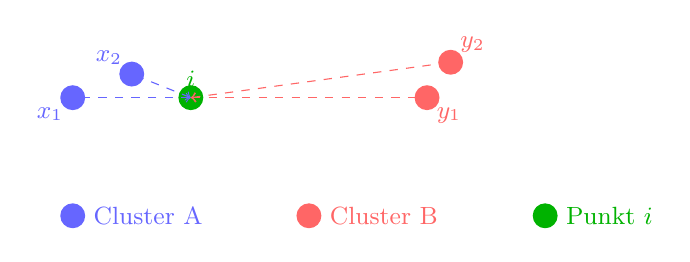
\begin{tikzpicture}[scale=1.5, every node/.style={font=\small}]
    % Cluster A (blau): zwei Punkte
    \fill[blue!60] (0,0) circle (3pt) node[below left] {$x_1$};
    \fill[blue!60] (0.5,0.2) circle (3pt) node[above left] {$x_2$};
    % Cluster B (rot): ein Punkt
    \fill[red!60] (3,0) circle (3pt) node[below right] {$y_1$};
    \fill[red!60] (3.2,0.3) circle (3pt) node[above right] {$y_2$};
    % Punkt i (grün)
    \coordinate (i) at (1,0);
    \fill[green!70!black] (i) circle (3pt) node[above] {$i$};

    % a(i)-Linien zu beiden A-Punkten
    \draw[blue!60, dashed, <->] (i) -- node[below] {} (0,0);
    \draw[blue!60, dashed, <->] (i) -- node[above] {} (0.5,0.2);

    % b(i)-Linie
    \draw[red!60, dashed, <->] (i) -- node[below] {} (3,0);
    \draw[red!60, dashed, <->] (i) -- node[above] {} (3.2,0.3);

    % Legende
    \begin{scope}[shift={(0,-1)}]
      \fill[blue!60] (0,0) circle (3pt) node[right=4pt] {Cluster A};
      \fill[red!60] (2,0) circle (3pt) node[right=4pt] {Cluster B};
      \fill[green!70!black] (4,0) circle (3pt) node[right=4pt] {Punkt $i$};
    \end{scope}
  \end{tikzpicture}
  \caption{Beispiel einer einfachen Clusterzuordnung}
  \label{fig:silhouette_example}
\end{figure}


\paragraph{Kritische Einordnung:}
Ein Nachteil des Silhouette‐Index ist, dass er runde und gleichmäßig dichte Cluster und runde
Cluster annimmt. Bei stark ungleich geformten oder  
verrauschten Clustern kann er daher irreführende Werte liefern (Siehe komplexeres Code-beispiel im verlinkten Beispiel mit halbmondförmigen Cluster: \url{https://github.com/Jens011203/Evaluierung_Integrationsseminar/blob/main/src/Clustering.ipynb}).
Außerdem reagiert er nicht auf Merkmals‑Bias: Trennt ein Algorithmus auf Basis irrelevanter Variablen,  
bleibt dies im Silhouette‑Score unentdeckt (vgl. \cite{Miller2024}). Deswegen wird diese Metrik vor allem genutzt wenn keine wahren labels in den Daten vorhanden sind.

\subsection{Davies-Bouldin-Index} Der \ac{DBI} misst
die Ähnlichkeit zwischen jedem
Cluster und dem ähnlichsten Fremdcluster. Für jeden Cluster $i$ definiert
man $s_i$ als den durchschnittlichen Abstand der Punkte von ihrem
Cluster-Zentroid (also die Varianz im Cluster), und für Clusterpaare $(i,j)$ den Abstand $d_{ij}$ zwischen
den Zentroiden. Dann berechnet man für jedes Paar $R_{ij} = (s_i + s_j)/d_{ij}$
und wählt für jeden Cluster $i$ den größten Wert $\max_{j\neq i} R_{ij}$. Der
Davies-Bouldin-Index ist das Mittel dieser Maxima: 
\[ DBI = \frac{1}{k}\sum_{i=1}^k \max_{j\neq i}\frac{s_i + s_j}{d_{ij}}, \]
mit $k$ der Anzahl der Cluster. Ein niedriger \ac{DBI} bedeutet bessere Cluster (maximale
Separation und geringe Streuung). Der Wert kann theoretisch bis $0$ reichen
(perfekte Trennung) (vgl. \cite{Davies1979} S.224f).

\paragraph{Beispiel:} Nehmen wir zwei Cluster mit Zentroiden \(c_1\) und \(c_2\),
deren Streuungen \(s_1=1\) und \(s_2=0{,}5\) sind, und Abstand \(d_{12}=2\). Dann ist
\[
R_{12}=\frac{s_1 + s_2}{d_{12}} = \frac{1 + 0.5}{2} = 0.75,
\]
was für dieses Paar den hohen Ähnlichkeitswert beiträgt und den DBI erhöht.
Befänden sich die Zentroiden jedoch bei \(d_{12}=5\), so wäre  
\[
R_{12} = \frac{1 + 0.5}{5} = 0.3,
\]
und der \ac{DBI} bliebe gering (gutes Clustering).

\paragraph{Kritische Einordnung:} Der \ac{DBI} ist ein effizientes, intrinsisches Maß, bei dem kleinere Werte
eine bessere Clusterstruktur anzeigen (Minimum = 0). Im Vergleich zum Silhouette‐Index ist die Berechnung
deutlich schneller und daher für großvolumige Datensätze sehr gut geeignet.
Nachteil: Er setzt euklidische Abstände zwischen Clusterzentroiden voraus und kann bei spärlichen oder
nicht‑euklidischen Daten irreführende Ergebnisse liefern, wenn alternative Distanzmaße besser zur Struktur der Daten passen.
(vgl. \cite{Miller2024}). Zudem kann er wie der Silhoutte-Koeffizient bei komplexeren Cluster-Strukturen verfälschte Werte liefern.

\subsection{Calinski-Harabasz-Index} Der Calinski-Harabasz-Index (auch Variance
Ratio Criterion) setzt die Streuung zwischen den Clustern ins Verhältnis zur
Streuung innerhalb der Cluster (vgl. \cite{Calinski1974}). Formal
sei $N$ die Gesamtzahl der Punkte, $k$ die Anzahl der Cluster, $B$ die
zwischen-Cluster-Varianz (Summe der quadrierten Abstände der Cluster-Zentren
zum Gesamtdurchschnitt) und $W$ die intra-Cluster-Varianz (Summe der
quadrierten Abstände der Punkte zu ihren jeweiligen Zentren). Dann ist der
CH-Index definiert als 
\[
CH 
= \frac{B/(k-1)}{W/(N-k)}
= \frac{B}{W} \cdot \frac{N - k}{k - 1}
\]
Ein höherer Wert
zeigt klarere Trennung und dichtere Cluster gute Klassifikation, während ein
kleinerer Wert auf schlechtere Partitionen (vgl. \cite{Calinski1974}). 

\paragraph{Beispiel:} Sind die Cluster perfekt kompakt ($W\to0$), wächst $CH$ ins
Unendliche. Bei nur einem Cluster ($k=1$) definiert man meist $CH=0$.
Üblicherweise wählt man das $k$, für das $CH$ am größten ist.

\paragraph{Kritische Einordnung:} Der CH-Index ist schnell berechenbar und eignet
sich für große Datensätze. Wie auch die anderen intrinsischen Metriken belohnt er kompakte, klar getrennte Cluster, kann
aber bei sehr vielen kleinen Clustern hohe Werten liefern und ist nur im
Vergleich unterschiedlicher $k$-Lösungen sinnvoll (vgl. \cite{Miller2024}).

\section{Extrinsische Metriken}

\subsection{Purity}
Die Purity eines Clusters \(C_i\) mit \(n_i\) Datenpunkten und
\(n_{h}^{(i)}\) Datenpunkten der dominanten (wahrheitsgemäßen) Klasse ist
definiert als {vgl. \cite{huang2008similarity} S.54}:
\[
  P(C_i)=\frac{1}{n_i}\max_h n_{h}^{(i)}.
\]
Der Gesamt‑Purity-Score eines Clusterings ist das gewichtete Mittel über alle \(k\) Cluster:
\[
  \text{Purity} = \sum_{i=1}^k \frac{n_i}{N}\,P(C_i).
\]

\paragraph{Beispiel:}  
Ein Vorgeschlagenes Cluster \(C_1\) enthält 10 Punkte, davon 7 aus Klasse A.
Dann gilt
\[
  P(C_1) = \frac{7}{10} = 0{,}7.
\]

\paragraph{Kritische Einordnung:}  
Purity ist sehr einfach und anschaulich, aber durch Einpunkt‑Cluster trivialisierbar und ignoriert Minderheitsklassen.
Zudem ist ein fairer Vergleich nur bei gleicher Anzahl \(k\) möglich.

\subsection{Adjusted Rand Index (ARI)}
Der \ac{ARI} beschreibt die Übereinstimmung zweier Cluster \(X\) (Vorhersage),
\(Y\) (\emph{Ground Truth}) und korrigiert um die erwartete Übereinstimmung
bei zufälliger Zuordnung (vgl. \cite{Hubert1985} S.194ff und \cite{Miller2024}):
\[
\mathrm{ARI}
= \frac{\mathrm{RI} - \mathbb{E}[\mathrm{RI}]}{1 - \mathbb{E}[\mathrm{RI}]},
\]
wobei der \emph{Rand‐Index}
\[
\mathrm{RI} = \frac{a + d}{\binom{n}{2}}
\]
den Anteil aller Paare misst, die in beiden Partitionen entweder im gleichen Cluster (\(a\)) oder in verschiedenen Clustern (\(d\)) liegen.  
Die Erwartung \(\mathbb{E}[\mathrm{RI}]\) unter zufälliger Clusterbildung berechnet sich aus den Clustergrößen in \(X\) und \(Y\):
\[
\mathbb{E}[\mathrm{RI}]
= \frac{\displaystyle\sum_i \binom{n_i^{(X)}}{2}\;\times\;\sum_j\binom{n_j^{(Y)}}{2}}{\binom{n}{2}^2},
\]
wobei \(n_i^{(X)}\) und \(n_j^{(Y)}\) die Größen der Cluster \(i\) in \(X\) bzw.\ \(j\) in \(Y\) sind.

\textbf{Wertebereich:} \(\mathrm{ARI}\in[-1,1]\), wobei  
\(\mathrm{ARI}=1\) perfekte Übereinstimmung,  
\(\mathrm{ARI}=0\) Zufallsniveau und  
\(\mathrm{ARI}<0\) schlechter als Zufall bedeutet.

\paragraph{Beispiel:}

Gegeben sind drei Objekte \(\{1,2,3\}\) mit  
\[
X:\{1,2\},\{3\}, 
\quad
Y:\{1\},\{2,3\}.
\]
Es existieren \(\binom{3}{2}=3\) Paare. Wir ermitteln
\[
a=0\quad(\text{kein Paar in beiden Partitionen im selben Cluster}),
\]
\[
d=1\quad(\text{z.\,B. Paar }(1,3)\text{ in beiden Partitionen getrennt}).
\]
Damit ist:
\[
\mathrm{RI}=\frac{a+d}{3}=\frac{0+1}{3}=\tfrac{1}{3}.
\]
Für die Erwartung unter Zufall:
\[
\sum_i\binom{n_i^{(X)}}{2}=1,\quad
\sum_j\binom{n_j^{(Y)}}{2}=1,
\quad
\mathbb{E}[\mathrm{RI}]=\frac{1\cdot1}{3^2}=\tfrac{1}{9}.
\]
Folglich
\[
\mathrm{ARI}
=\frac{\tfrac13-\tfrac19}{1-\tfrac19}
=\frac{\tfrac{2}{9}}{\tfrac{8}{9}}
=\tfrac{1}{4}
=0{,}25.
\]

\paragraph{Kritische Einordnung:}  
\ac{ARI} ist eine sehr häufig verwendete und zuverlässige Metrik. Wie bei allen extrinsischen Metriken ist hier zur Bewertung eine \textit{Ground Truth}
notwendig. Eine weitere Einschränkung beim \ac{ARI} ist die Verzerrung bezüglich der Clustergröße. 
Wenn eine Clustering-Lösung eine Mischung aus großen und kleinen Clustern enthält, wird \ac{ARI} vorwiegend von den großen Clustern beeinflusst (vgl. \cite{Miller2024}).

\subsection{Adjusted Mutual Information (AMI)}
Die \ac{AMI} beschreibt wie viel Information zwischen der dem vorhergesagten
Cluster \(X\) und den tatsächlichen Cluster Y geteilt wird und korrigiert für
zufällige Übereinstimmungen. 
Die Metrik hat denselben Wertebereich wie \ac{ARI} und wird wie folgt bestimmt (vgl. \cite{Miller2024}):
\[
\mathrm{AMI}(X,Y) = \frac{\mathrm{MI}(X,Y) - \mathbb{E}[\mathrm{MI}(X,Y)]}{\mathrm{avg}(H(X),H(Y)) - \mathbb{E}[\mathrm{MI}(X,Y)]},
\]
wobei:
\begin{itemize}
    \item $H$ = individuelle Entropie -- ein Maß für die erwartete Unsicherheit
    \item $\mathrm{MI}$ = Der Mutual-Information-Algorithmus 
    \item $\mathbb{E}$ = der Erwartungswert basierend auf Zufall
\end{itemize}

\paragraph{Beispiel:}
Gegeben sind die Clusterings \(X: \{A,B\}, \{C\}\) und \(Y: \{A\}, \{B,C\}\).
Würde man hiervon die \ac{MI} berechnen erhält man \(MI = 0{,}251\). 
Nach Korrektur um den Zufallswert erhält man \(\mathrm{AMI}(X,Y) = 0{,}136\), was etwas besser als 0 (zufällig) ist.

\paragraph{Kritische Einordnung:}
\ac{AMI} bietet durch die Zufallskorrektur eine robustere Interpretation als
die einfache \ac{MI}. Ein wesentlicher Unterschied zu \ac{ARI} liegt in den
jeweiligen Verzerrungen: Während \ac{ARI} Lösungen mit ähnlich großen Clustern
bevorzugt, ist \ac{AMI} zu „reinen“ Clustern verzerrt, die nur einen Klassentyp
enthalten und oft unausgewogen sind (vgl. \cite{Miller2024}). 
